\chapter{Le CTF}

\section{Définition}

Un CTF\footnote{CTF peut-être traduit en capture du drapeau.} ou "Capture The Flag" est une activité consistant à s'introduire dans une machine cible vulnérable pour y trouver un drapeau en guise de victoire. Les possibilités de CTF sont extrêmement vastes et ces dernières nécessitent des connaissances dans de multiples domaines. C'est pour cette raison que nous allons nous concentrer sur les CTFs "Web" afin de pouvoir exploiter complètement vos connaissances en sortie d'IUT R\&T. 

Avant de commencer à vous présenter des attaques bien précises, nous allons vous expliquer les différents angles d'attaques que nous pouvons retrouver généralement lors d'un CTF. En effet, il y a toujours un "protocole" à suivre lors de la réalisation d'une attaque qui va nous permettre de résoudre un CTF. Ce protocole se divise en trois grandes phases qui sont :
\begin{itemize}
    \item La collecte d'informations
    \item L'exploitation de ces informations via des failles
    \item L'intrusion dans le système cible avec possibilité de devenir administrateur\\
\end{itemize}

Chacune de ces phases contient des sous-phases en fontion des outils utilisés et donc des failles. Comme vous pouvez le voir sur le schéma indiqué dans la \textbf{figure \ref{fig:schema-ctf}}, une attaque est coupée en trois parties. La première qui se nomme "Recherche d'informations active". C'est une sous-catégorie de la recherche d'informations. En effet, au sein de ce schéma, on va considérer que la recherche d'informations passive a déjà été effectuée car elle n'est pas obligatoire. La deuxième phase nous présente les outils que nous utilisons en général pour utiliser les informations récupérées via la phase précédente et ainsi exploiter des failles. Ces trois outils sont les suivants : Burpsuite, SQLMAP et Metasploit. Burpsuite va être utilisé pour contourner des restrictions dans un formulaire via son proxy et ainsi permettre la création d'un reverse-shell par exemple. SQLMAP va nous permettre d'exploiter des failles SQL et ainsi dévoiler une base de données. Metasploit est quant à lui beaucoup plus complexe. En effet, l'ensemble d'un CTF pourrait être entièrement réalisé avec cet outil car il regroupe l'ensemble des outils de pentest ainsi que d'autres modules tel que Meterpreter. Le but de cette phase est donc d'obtenir directement un reverse-shell ou bien des informations qui pourraient être cryptées. C'est donc à partir de ce moment qu'il faudra choisir la branche adéquate pour réaliser son CTF.

\begin{figure}[htp!]
  \centering
  \setlength\figureheight{7cm}
  \setlength\figurewidth{9cm}
  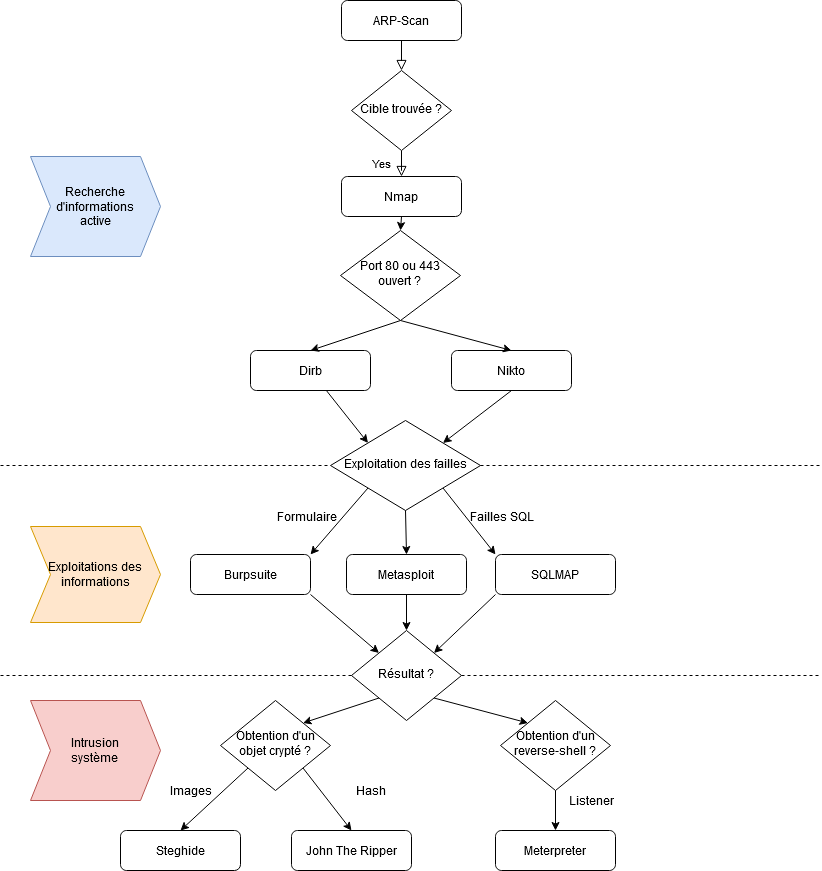
\includegraphics[width=1\textwidth]{oui/images/Chapitre1/Attackdiag.png}
  \caption{Schéma d'attaque d'un CTF}
  \label{fig:schema-ctf}
\end{figure}

Comme on a pu le comprendre, aucune attaque n'est la même et c'est en pratiquant que l'on peut comprendre pourquoi utiliser un outil plutôt qu'un autre. Cependant, avant d'utiliser ces outils, nous allons nous pencher sur notre environnement de travail.

\section{Environnement de travail}

\subsection{Kali Linux}

Kali Linux est une distribution Linux, basée sur Debian, orientée sur la sécurité informatique. Anciennement BackTrack, cette distribution a su se réinventer en devenant Kali et ainsi regrouper un nombre « incalculable » de logiciels conçus pour la sécurité et l’intrusion informatique. C’est pour cette raison que nous avons choisi de travailler sur cette distribution afin d'effectuer des CTF.

\subsection{Mise en place d'un CTF}

Pour commencer un CTF, il nous faut aller chercher une machine virtuelle attaquable. Pour cela, nous pouvons aller sur le site de Vulnhub et récupérer un fichier avec l’extension .OVA. Vulnhub est un site répertoriant des CTFs créés par la communauté. Il est donc très facile de s'exercer via ce site.\\
Ce fichier OVA contient notre machine cible que l’on pourra allumer sous Virtualbox comme vu en \textbf{figure \ref{fig:import-ova}}.

\begin{figure}[htp!]
  \centering
  \setlength\figureheight{7cm}
  \setlength\figurewidth{9cm}
  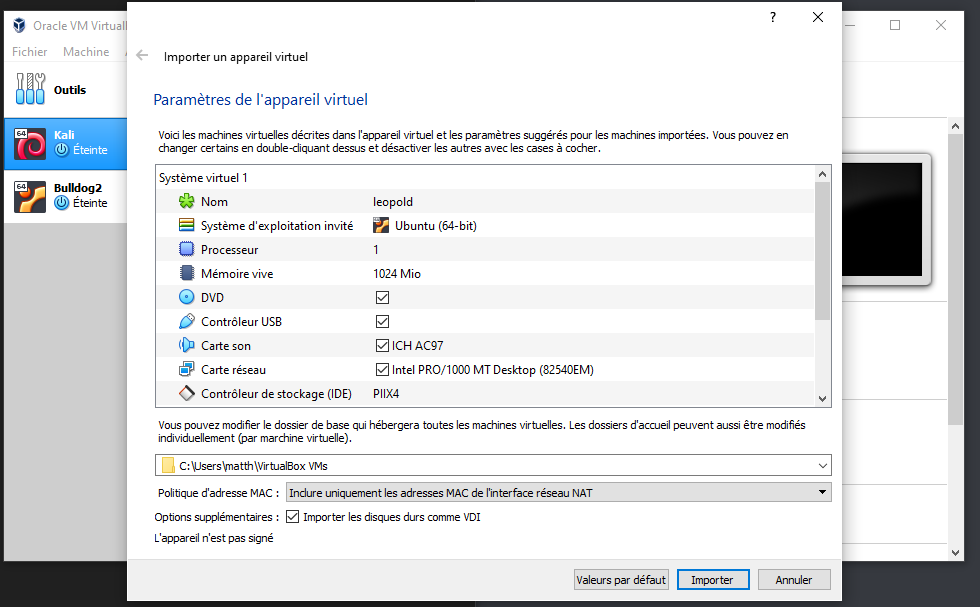
\includegraphics[width=0.77\textwidth]{oui/images/Chapitre1/importation.png}
  \caption{Imporation d'un CTF}
  \label{fig:import-ova}
\end{figure}

Après avoir réalisé cette étape, vous pourrez aller vous occuper des interfaces réseaux de votre Kali et de votre CTF afin qu'il puisse communiquer entre eux. En général, le CTF sera configuré en dhcp ce qui vous permettra d'utiliser le réseau NAT ou bien le mode Pont/Bridge. Pour rappel, le réseau NAT sous Virtualbox créé un routeur et un service DHCP entre votre ordinateur et votre machine virtuelle. Ainsi, cette dernière a accès à internet et à son propre réseau. Le mode Pont va vous permettre d'annoncer votre machine virtuelle comme machine à part entière sur votre réseau. Ainsi, la VM pourra communiquer sur votre réseau et obtenir via DHCP une adresse si le service est activé sur le réseau. Dans les deux cas, pensez à mettre votre machine attaquante et cible dans le même réseau. Une fois que cette configuration est faite, vous pourrez allumer vos machines et commencer votre attaque tout en respectant l'ordre d'attaque.